\documentclass{article}
\usepackage[utf8x]{inputenc}
\usepackage{ucs}
\usepackage{amsmath} 
\usepackage{amsfonts}
\usepackage{upgreek}
\usepackage[english,russian]{babel}
\usepackage{graphicx}
\usepackage{float}
\usepackage{textcomp}
\usepackage{hyperref}
\usepackage{geometry}
  \geometry{left=2cm}
  \geometry{right=1.5cm}
  \geometry{top=1cm}
  \geometry{bottom=2cm}
\usepackage{tikz}
\usepackage{ccaption}
\usepackage{multicol}

\usepackage{listings}
%\setlength{\columnsep}{1.5cm}
%\setlength{\columnseprule}{0.2pt}


\definecolor{solcolor}{RGB}{226,240,245}

\begin{document}
\pagenumbering{gobble}

\lstset{
  language=C,                % choose the language of the code
  basicstyle=\linespread{1.1}\ttfamily,
  columns=fixed,
  fontadjust=true,
  basewidth=0.5em,
  keywordstyle=\color{blue}\bfseries,
  commentstyle=\color{gray},
  stringstyle=\ttfamily\color{orange!50!black},
  showstringspaces=false,
  %numbers=false,                   % where to put the line-numbers
  numbersep=5pt,
  numberstyle=\tiny\color{black},
  numberfirstline=true,
  stepnumber=1,                   % the step between two line-numbers.        
  numbersep=10pt,                  % how far the line-numbers are from the code
  backgroundcolor=\color{white},  % choose the background color. You must add \usepackage{color}
  showstringspaces=false,         % underline spaces within strings
  captionpos=b,                   % sets the caption-position to bottom
  breaklines=true,                % sets automatic line breaking
  breakatwhitespace=true,         % sets if automatic breaks should only happen at whitespace
  xleftmargin=.2in,
  extendedchars=\true,
  keepspaces = true,
  frame=tlbr,
  framesep=14pt,
  framerule=0pt,
}
\lstset{literate=%
   *{0}{{{\color{red!20!violet}0}}}1
    {1}{{{\color{red!20!violet}1}}}1
    {2}{{{\color{red!20!violet}2}}}1
    {3}{{{\color{red!20!violet}3}}}1
    {4}{{{\color{red!20!violet}4}}}1
    {5}{{{\color{red!20!violet}5}}}1
    {6}{{{\color{red!20!violet}6}}}1
    {7}{{{\color{red!20!violet}7}}}1
    {8}{{{\color{red!20!violet}8}}}1
    {9}{{{\color{red!20!violet}9}}}1
}

\title{Семинар \#3: Массивы. \vspace{-5ex}}\date{}\maketitle
\section*{Часть 1: Основы работы с массивом}
Создаём массив из шести элементов и печатаем элемент с индексом \texttt{1}, то есть число \texttt{8}.
\begin{lstlisting}
#include <stdio.h>
int main() {
	int a[6] = {4, 8, 15, 16, 23, 42};
	printf("%d\n", a[1]);
}
\end{lstlisting}
\begin{center}
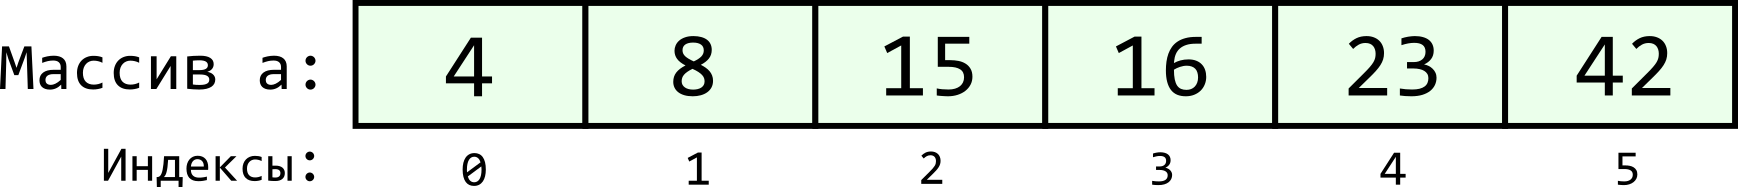
\includegraphics[scale=1]{../images/array_indexes.png}
\end{center}

\subsubsection*{Задачи:}
\begin{itemize}
\item Напечатайте первый элемент массива (то есть число \texttt{4}).
\item Напечатайте сумму двух послених элементов массива.
\item Измените элемент с индексом \texttt{1} с \texttt{8} на \texttt{20} и напечатайте его. Чтобы изменить элемент массива:
\begin{lstlisting}
a[1] = 20;
\end{lstlisting}
\end{itemize}
\begin{lstlisting}[backgroundcolor = \color{solcolor}]
#include <stdio.h>
int main() {
	int a[6] = {4, 8, 15, 16, 23, 42};
	printf("%d\n", a[0]);
	printf("%d\n", a[4] + a[5]);
	a[1] = 20;
	printf("%d\n", a[1]);
}
\end{lstlisting}

\subsection*{Работа с элементами массива в цикле}
Часто к элементам массива необходимо обращаться в цикле. Пример программы, которая прибавляет \texttt{1} к каждому элементу массива \texttt{a} и печатает этот массив.
\begin{lstlisting}
#include <stdio.h>
int main() {
    int a[6] = {4, 8, 15, 16, 23, 42};
    for (int i = 0; i < 6; ++i) {
        a[i] += 1;
    }
    for (int i = 0; i < 6; ++i) {
        printf("%d ", a[i]);
    }
}
\end{lstlisting}
\subsubsection*{Задачи:}
\begin{itemize}
\item Напечатайте массив \texttt{a} так, чтобы элементы были разделены запятыми.
\begin{lstlisting}[backgroundcolor = \color{solcolor}]
#include <stdio.h>
int main() {
    int a[6] = {4, 8, 15, 16, 23, 42};
    for (int i = 0; i < 6; ++i) {
        printf("%d, ", a[i]);
    }
}
\end{lstlisting}
\item Напечатайте массив \texttt{a} так, чтобы каждый элемент печатался в новой строке.
\begin{lstlisting}[backgroundcolor = \color{solcolor}]
#include <stdio.h>
int main() {
    int a[6] = {4, 8, 15, 16, 23, 42};
    for (int i = 0; i < 6; ++i) {
        printf("%d\n", a[i]);
    }
}
\end{lstlisting}
\item Напечатайте массив \texttt{a} два раза (через пробел).
\begin{lstlisting}[backgroundcolor = \color{solcolor}]
#include <stdio.h>
int main() {
    int a[6] = {4, 8, 15, 16, 23, 42};
    for (int i = 0; i < 6; ++i) {
        printf("%d ", a[i]);
    }
    for (int i = 0; i < 6; ++i) {
        printf("%d ", a[i]);
    }
}
\end{lstlisting}
Или так:
\begin{lstlisting}[backgroundcolor = \color{solcolor}]
#include <stdio.h>
int main() {
    int a[6] = {4, 8, 15, 16, 23, 42};
    for (int j = 0; j < 2; ++j) {
        for (int i = 0; i < 6; ++i) {
            printf("%d ", a[i]);
        }
    }
}
\end{lstlisting}

\item Напечатайте каждый второй элемент массива \texttt{a}. (Получится \texttt{4 15 23}).
\begin{lstlisting}[backgroundcolor = \color{solcolor}]
#include <stdio.h>
int main() {
    int a[6] = {4, 8, 15, 16, 23, 42};
    for (int i = 0; i < 6; i += 2) {
        printf("%d ", a[i]);
    }
}
\end{lstlisting}
\item Напечатайте все чётные элементы массива \texttt{a}. (\texttt{4 8 16 42}).
\begin{lstlisting}[backgroundcolor = \color{solcolor}]
#include <stdio.h>
int main() {
    int a[6] = {4, 8, 15, 16, 23, 42};
    for (int i = 0; i < 6; i++) {
        if (a[i] % 2 == 0)
            printf("%d ", a[i]);
    }
}
\end{lstlisting}
\item Напечатайте массив \texttt{a} наоборот. (\texttt{42 23 16 15 8 4}).\\
Вариант 1:
\begin{lstlisting}[backgroundcolor = \color{solcolor}]
#include <stdio.h>
int main() {
    int a[6] = {4, 8, 15, 16, 23, 42};
    for (int i = 5; i >= 0; i--) {
        printf("%d ", a[i]);
    }
}
\end{lstlisting}
Вариант 2:
\begin{lstlisting}[backgroundcolor = \color{solcolor}]
#include <stdio.h>
int main() {
    int a[6] = {4, 8, 15, 16, 23, 42};
    for (int i = 0; i < 6; i++) {
        printf("%d ", a[5 - i]);
    }
}
\end{lstlisting}

\newpage
\item Напечатайте каждый второй элемент массива \texttt{a} наоборот. (\texttt{42 16 8}).
\begin{lstlisting}[backgroundcolor = \color{solcolor}]
#include <stdio.h>
int main() {
    int a[6] = {4, 8, 15, 16, 23, 42};
    for (int i = 5; i >= 0; i -= 2) {
        printf("%d ", a[i]);
    }
}
\end{lstlisting}
\item Напечатайте индексы и элементы массива в следующем формате:
\begin{verbatim}
0:  4
1:  8
2: 15
3: 16
4: 23
5: 42
\end{verbatim}
Для печати используйте \texttt{\%2d} или \texttt{\%02d}.
\begin{lstlisting}[backgroundcolor = \color{solcolor}]
#include <stdio.h>
int main() {
    int a[6] = {4, 8, 15, 16, 23, 42};
    for (int i = 0; i < 6; i++) {
        printf("%d: %2d\n", i, a[i]);
    }
}
\end{lstlisting}
\item Напечатайте все элементы массива, умноженные на \texttt{2}, не меняя массив.\\
\begin{lstlisting}[backgroundcolor = \color{solcolor}]
#include <stdio.h>
int main() {
    int a[6] = {4, 8, 15, 16, 23, 42};
    for (int i = 0; i < 6; i++) {
        printf("%d ", 2 * a[i]);
    }
}
\end{lstlisting}
\end{itemize}
\newpage
Во всех следующих задачах нужно сначала менять сам массив, а затем печатать его элементы.
\begin{itemize}
\item Измените массив, умножив все его элементы на \texttt{2}. Напечатайте его.
\begin{lstlisting}[backgroundcolor = \color{solcolor}]
#include <stdio.h>
int main() {
    int a[6] = {4, 8, 15, 16, 23, 42};
    for (int i = 0; i < 6; i++) {
        a[i] *= 2;
    }
    for (int i = 0; i < 6; i++) {
        printf("%d ", a[i]);
    }
}
\end{lstlisting}
\item Прибавьте к элементам изначального массива \texttt{a} их индексы и напечатайте массив. Должно получиться:
\begin{verbatim}
4 9 17 19 27 47
\end{verbatim}
\begin{lstlisting}[backgroundcolor = \color{solcolor}]
#include <stdio.h>
int main() {
    int a[6] = {4, 8, 15, 16, 23, 42};
    for (int i = 0; i < 6; i++) {
        a[i] += i;
    }
    for (int i = 0; i < 6; i++) {
        printf("%d ", a[i]);
    }
}
\end{lstlisting}
\item Измените изначальный массив \texttt{a} следующим образом:
\begin{itemize}
\item Если число чётное, то его нужно разделить на \texttt{2}
\item Если число нечётное, то его нужно умножить на \texttt{3} и прибавить 1
\end{itemize}
Напечатайте этот массив. Должно получиться:
\begin{verbatim}
2 4 46 8 70 21
\end{verbatim}
\begin{lstlisting}[backgroundcolor = \color{solcolor}]
#include <stdio.h>
int main() {
    int a[6] = {4, 8, 15, 16, 23, 42};
    for (int i = 0; i < 6; i++) {
        if (a[i] % 2)
            a[i] = 3 * a[i] + 1;
        else
            a[i] /= 2;
    }
    for (int i = 0; i < 6; i++) {
        printf("%d ", a[i]);
    }
}
\end{lstlisting}
Вариант 2 (с использованием тернарного оператора):
\begin{lstlisting}[backgroundcolor = \color{solcolor}]
#include <stdio.h>
int main() {
    int a[6] = {4, 8, 15, 16, 23, 42};
    for (int i = 0; i < 6; i++) {
    	a[i] = (a[i] % 2) ? 3 * a[i] + 1 : a[i] / 2;
    }
    for (int i = 0; i < 6; i++) {
        printf("%d ", a[i]);
    }
}
\end{lstlisting}
\end{itemize}


\subsection*{Считывание элементов массива в цикле}
Считывать нужно каждый элемент массив по отдельности в цикле. Но тут возникает проблема: мы не знаем количество элементов, которые придут на вход. Поэтому сначала мы считываем количество элементов \texttt{n}. Тут возникает ещё одна проблема: очень нежелательно создавать массив переменной длины. То есть не нужно писать так:
\begin{lstlisting}
int n = 10;
int a[n];
\end{lstlisting}
Некоторые компиляторы \texttt{С/C++} это поддерживают, а некоторые нет. Поэтому лучше создать массив побольше и работать с ним. Пример программы, которая считывает массив и печатает его:
\begin{lstlisting}
#include <stdio.h>
int main() {
    int n;
    scanf("%d", &n);
    int a[1000];
    for (int i = 0; i < n; ++i) {
        scanf("%d", &a[i]);
    }
    
    for (int i = 0; i < n; ++i) {
        printf("%d ", a[i]);
    }    
}
\end{lstlisting}

\newpage
\subsubsection*{Задачи:}
\begin{itemize}
\item Считайте массив и напечатайте его \texttt{2} раза.
\begin{center}
\begin{tabular}{ l | l }
 вход & выход \\ \hline
 \texttt{3} & \texttt{1 6 2 1 6 2}  \\ 
 \texttt{1 6 2} &   \\
\end{tabular}
\end{center}
\begin{lstlisting}[backgroundcolor = \color{solcolor}]
#include <stdio.h>
int main() {
    int n;
    scanf("%d", &n);
    int a[1000];
    for (int i = 0; i < n; ++i) {
        scanf("%d", &a[i]);
    }
    for (int j = 0; j < 2; ++j) {
        for (int i = 0; i < n; ++i) {
            printf("%d ", a[i]);
        }
    }
}
\end{lstlisting}


\item Считайте массив и напечатайте его в обратном порядке.
\begin{center}
\begin{tabular}{ l | l }
 вход & выход \\ \hline
 \texttt{4} & \texttt{6 4 7 1}  \\ 
 \texttt{1 7 4 6} &   \\
\end{tabular}
\end{center}
\begin{lstlisting}[backgroundcolor = \color{solcolor}]
#include <stdio.h>
int main() {
    int n;
    scanf("%d", &n);
    int a[1000];
    for (int i = 0; i < n; ++i) {
        scanf("%d", &a[i]);
    }
    for (int i = n - 1; i >= 0; --i) {
        printf("%d ", a[i]);
    }
}
\end{lstlisting}

\item Сдвиньте все элементы массива \texttt{a} вправо на \texttt{1}. Первый элемент должен стать вторым, второй первым третьим, ... последний первым. Сначала нужно изменить массив, а потом напечатать его.
\begin{center}
\begin{tabular}{ l | l }
 вход & выход \\ \hline
 \texttt{5} & \texttt{1 4 2 9 6}  \\ 
 \texttt{4 2 9 6 1} &   \\
\end{tabular}
\end{center}

\begin{lstlisting}[backgroundcolor = \color{solcolor}]
#include <stdio.h>
int main() {
    int n;
    scanf("%d", &n);
    int a[1000];
    for (int i = 0; i < n; ++i) {
        scanf("%d", &a[i]);
    }
    int temp = a[n - 1];
    for (int i = n - 1; i > 0; --i) {
        a[i] = a[i - 1];
    }
    a[0] = temp;
    for (int i = 0; i < n; ++i) {
        printf("%d ", a[i]);
    }
}
\end{lstlisting}

\item Поменяйте местами соседей. То есть первый элемент меняется со вторым, третий с четвёртым. Если количество элементов нечётно, то последний элемент не меняется. Сначала нужно изменить массив, а потом напечатать его.
\begin{center}
\begin{tabular}{ l | l }
 вход & выход \\ \hline
 \texttt{6} & \texttt{2 1 4 3 6 5}  \\ 
 \texttt{1 2 3 4 5 6} &   \\ \hline
 \texttt{5} & \texttt{2 4 6 9 1}  \\ 
 \texttt{4 2 9 6 1} &   \\
\end{tabular}
\end{center}
\begin{lstlisting}[backgroundcolor = \color{solcolor}]
#include <stdio.h>
int main() {
    int n;
    scanf("%d", &n);
    int a[1000];
    for (int i = 0; i < n; ++i) {
        scanf("%d", &a[i]);
    }
    for (int i = 0; i < n - 1; i += 2) {
        int temp = a[i];
        a[i] = a[i + 1];
        a[i + 1] = temp;
    }
    for (int i = 0; i < n; ++i) {
        printf("%d ", a[i]);
    }
}
\end{lstlisting}


\item Обратите массив. То есть первый элемент должен стать последним, а последний первым. Второй -- предпоследним, а предпоследний -- вторым и т.д. Сначала нужно изменить массив, а потом напечатать его.
\begin{center}
\begin{tabular}{ l | l }
 вход & выход \\ \hline
 \texttt{6} & \texttt{6 5 4 3 2 1}  \\ 
 \texttt{1 2 3 4 5 6} &   \\ \hline
 \texttt{3} & \texttt{2 4 7}  \\ 
 \texttt{7 4 2} &   \\
\end{tabular}
\end{center}

\begin{lstlisting}[backgroundcolor = \color{solcolor}]
#include <stdio.h>
int main() {
    int n;
    scanf("%d", &n);
    int a[1000];
    for (int i = 0; i < n; ++i) {
        scanf("%d", &a[i]);
    }
    for (int i = 0; i < n / 2; i++) {
        int temp = a[i];
        a[i] = a[n - 1 - i];
        a[n - 1 - i] = temp;
    }
    for (int i = 0; i < n; ++i) {
        printf("%d ", a[i]);
    }
}
\end{lstlisting}

\newpage
\item На вход подаётся массив, нужно применить к каждому элементу функцию факториала:
\begin{lstlisting}
int fact(int n) {
    int result = 1;
    for (int i = 1; i <= n; ++i) {
        result *= i;
    }
    return result;
}

\end{lstlisting}
Сначала нужно напечатать сами элементы в строку, а затем значения функции факториала.
\begin{center}
\begin{tabular}{ l | l }
 вход & выход \\ \hline
 \texttt{5} &           \texttt{3 1 \space\space5 0 \space4}  \\ 
 \texttt{3 1 5 0 4} &   \texttt{6 1 120 1 24}\\
\end{tabular}
\end{center}
\begin{lstlisting}[backgroundcolor = \color{solcolor}]
#include <stdio.h>
int fact(int n) {
    int result = 1;
    for (int i = 1; i <= n; ++i) {
        result *= i;
    }
    return result;
}

int main() {
    int n;
    scanf("%d", &n);
    int a[1000];
    for (int i = 0; i < n; ++i) {
        scanf("%d", &a[i]);
    }
    for (int i = 0; i < n; ++i) {
        printf("%-3d ", a[i]);
    }
    printf("\n");
    for (int i = 0; i < n; ++i) {
        printf("%-3d ", fact(a[i]));
    }
}
\end{lstlisting}

\end{itemize}

\newpage
\section*{Часть 2: Основные алгоритмы}
\subsection*{Поиск максимума}
Пример программы, которая считывает массив и печатает максимальный элемент. ($n \ge 1$).
\begin{lstlisting}
#include <stdio.h>
int main() {
    int n;
    scanf("%d", &n);
    int a[1000];
    for (int i = 0; i < n; ++i) {
        scanf("%d", &a[i]);
    }
    int max = a[0];
    for (int i = 1; i < n; ++i) {
        if (a[i] > max)
            max = a[i];
    }
    printf("%d\n", max); 
}
\end{lstlisting}



\begin{itemize}
\item Измените программу выше так, чтобы программа искала не максимум, а индекс максимального элемента
\begin{center}
\begin{tabular}{ l | l }
 вход & выход \\ \hline
 \texttt{6} & \texttt{4}  \\ 
 \texttt{7 1 5 2 9 5} &   \\ \hline
 \texttt{3} & \texttt{1}  \\ 
 \texttt{5 7 4} &   \\ \hline
 \texttt{1} & \texttt{0}  \\ 
 \texttt{1} &   \\
\end{tabular}
\end{center}
\begin{lstlisting}[backgroundcolor = \color{solcolor}]
#include <stdio.h>
int main() {
    int n;
    scanf("%d", &n);
    int a[1000];
    for (int i = 0; i < n; ++i) {
        scanf("%d", &a[i]);
    }
    int max_i = 0;
    for (int i = 1; i < n; ++i) {
        if (a[i] > a[max_i])
            max_i = i;
    }
    printf("%d\n", max_i); 
}
\end{lstlisting}

\newpage
\item Измените программу выше так, чтобы программа меняла местами максимальный и первый элементы.
\begin{center}
\begin{tabular}{ l | l }
 вход & выход \\ \hline
 \texttt{6} & \texttt{9 1 5 2 7 5}  \\ 
 \texttt{7 1 5 2 9 5} &   \\ \hline
 \texttt{3} & \texttt{7 5 4}  \\ 
 \texttt{5 7 4} &   \\ \hline
 \texttt{1} & \texttt{1}  \\ 
 \texttt{1} &   \\
\end{tabular}
\end{center}

\begin{lstlisting}[backgroundcolor = \color{solcolor}]
#include <stdio.h>
int main() {
    int n;
    scanf("%d", &n);
    int a[1000];
    for (int i = 0; i < n; ++i) {
        scanf("%d", &a[i]);
    }
    int max_i = 0;
    for (int i = 1; i < n; ++i) {
        if (a[i] > a[max_i])
            max_i = i;
    }
    int temp = a[max_i];
    a[max_i] = a[0];
    a[0] = temp;
    for (int i = 0; i < n; ++i) {
        printf("%d ", a[i]); 
    }
}
\end{lstlisting}

\newpage
\item \textbf{Поиск элемента в массиве.} На вход поступает массив и некоторое число. Нужно напечатать индекс этого числа в массиве или \texttt{-1} если такого элемента в массиве нет. Если элементов несколько, то нужно напечатать индекс первого из них.
\begin{center}
\begin{tabular}{ l | l }
 вход & выход \\ \hline
 \texttt{6} & \texttt{2}  \\ 
 \texttt{7 1 5 2 9 5} &   \\
 \texttt{5} &   \\ \hline

 \texttt{6} & \texttt{-1}  \\ 
 \texttt{7 1 5 2 9 5} &   \\
 \texttt{4} &   \\ \hline
 
 \texttt{1} & \texttt{0}  \\ 
 \texttt{1} &   \\
 \texttt{1} &   \\
\end{tabular}
\end{center}
\begin{lstlisting}[backgroundcolor = \color{solcolor}]
#include <stdio.h>
int main() {
    int n;
    scanf("%d", &n);
    int a[1000];
    for (int i = 0; i < n; ++i) {
        scanf("%d", &a[i]);
    }
    int x;
    scanf("%d", &x);
    
    int result = -1;
    for (int i = 0; i < n; ++i) {
        if (a[i] == x) {
            result = i;
            break;
        }
    }

    printf("%d ", result); 
}
\end{lstlisting}

\end{itemize}

\newpage
\subsection*{Алгоритмы на подмассивах}
Подмассив - это некоторая последовательная часть массива. Будем обозначать подмассив \texttt{a[l, r]} такую часть массива, элементы которого имеют индекс \texttt{i} в диапазоне \texttt{l <= i < r}. Обратите внимание, что мы договорились, что элемент \texttt{a[r]} не входит в подмассив \texttt{a[l, r]}.\\

Например, в подмассив \texttt{[1, 4]} массива \texttt{a} входят элементы \texttt{8, 15, 16}, а элемент \texttt{23} не входит.
\begin{center}
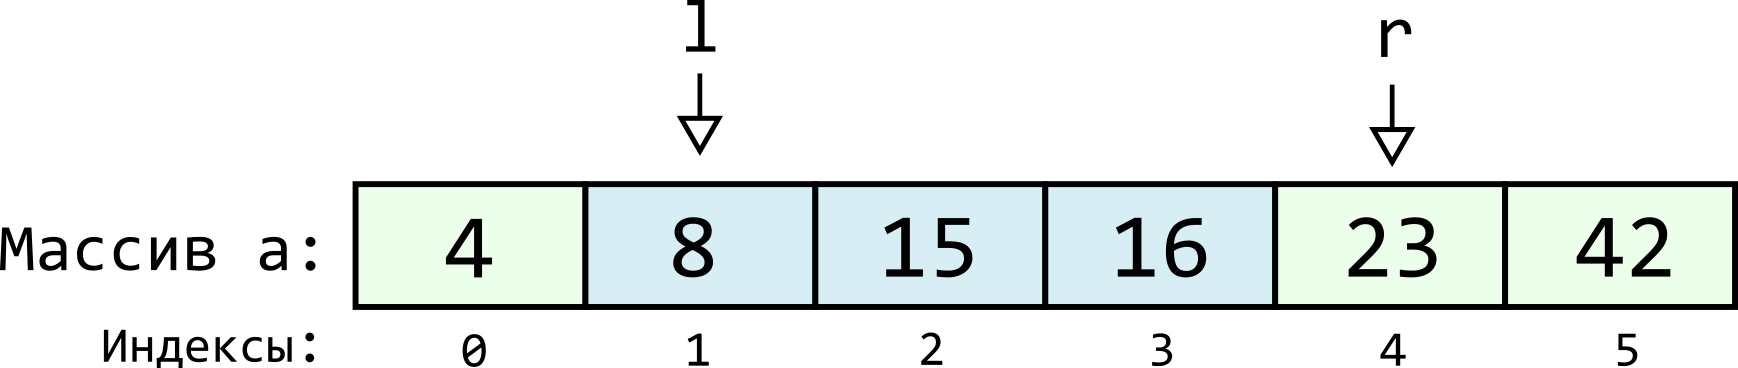
\includegraphics[scale=1]{../images/array_slice.png}
\end{center}

Пример программы, которая считывает массив и границы подмассива в этом массиве и печатает этот подмассив.
\begin{lstlisting}
#include <stdio.h>
int main() {
    int n;
    scanf("%d", &n);
    int a[1000];
    for (int i = 0; i < n; ++i) {
        scanf("%d", &a[i]);
    }
    int l, r;
    scanf("%d%d", &l, &r);

    for (int i = l; i < r; ++i) {
        printf("%d\n", a[i]); 
    }
}
\end{lstlisting}

\newpage
\begin{itemize}
\item Измените программу выше так, чтобы программа печатала сумму подмассива
\begin{center}
\begin{tabular}{ l | l }
 вход & выход \\ \hline
 \texttt{6} & \texttt{15}  \\ 
 \texttt{7 1 5 9 2 5} &   \\ 
 \texttt{1 4} &   \\ 
\end{tabular}
\end{center}

\begin{lstlisting}[backgroundcolor = \color{solcolor}]
#include <stdio.h>
int main() {
    int n;
    scanf("%d", &n);
    int a[1000];
    for (int i = 0; i < n; ++i) {
        scanf("%d", &a[i]);
    }
    int l, r;
    scanf("%d%d", &l, &r);
    int sum = 0;
    for (int i = l; i < r; ++i) {
        sum += a[i]; 
    }
    printf("%d\n", sum);
}
\end{lstlisting}

\item Измените программу выше так, чтобы программа находила индекс минимального элемента на подмассиве
\begin{center}
\begin{tabular}{ l | l }
 вход & выход \\ \hline
 \texttt{6} & \texttt{4}  \\ 
 \texttt{7 1 5 9 2 5} &   \\ 
 \texttt{2 6} &   \\ 
\end{tabular}
\end{center}

\begin{lstlisting}[backgroundcolor = \color{solcolor}]
#include <stdio.h>
int main() {
    int n;
    scanf("%d", &n);
    int a[1000];
    for (int i = 0; i < n; ++i) {
        scanf("%d", &a[i]);
    }
    int l, r;
    scanf("%d%d", &l, &r);
    int min_i = l;
    for (int i = l; i < r; ++i) {
        if (a[i] < a[min_i])
            min_i = i;
    }
    printf("%d\n", min_i);
}
\end{lstlisting}


\newpage
\item Измените программу выше так, чтобы программа меняла местами минимальный и первый элемент подмассива
\begin{center}
\begin{tabular}{ l | l }
 вход & выход \\ \hline
 \texttt{6} & \texttt{7 1 2 5 9 5}  \\ 
 \texttt{7 1 2 9 5 5} &   \\ 
 \texttt{3 6} &   \\ 
\end{tabular}
\end{center}

\begin{lstlisting}[backgroundcolor = \color{solcolor}]
#include <stdio.h>
int main() {
    int n;
    scanf("%d", &n);
    int a[1000];
    for (int i = 0; i < n; ++i) {
        scanf("%d", &a[i]);
    }
    int l, r;
    scanf("%d%d", &l, &r);
    int min_i = l;
    for (int i = l; i < r; ++i) {
        if (a[i] < a[min_i])
            min_i = i;
    }
    int temp = a[min_i];
    a[min_i] = a[l];
    a[l] = temp;
    for (int i = 0; i < n; ++i) {
        printf("%d ", a[i]);
    } 
}
\end{lstlisting}
\end{itemize}

\newpage
\subsection*{Сортировка}
Сортировка -- это упорядочение элементов по возрастанию, убыванию или по какому-то другому критерию.
\begin{itemize}
\item \textbf{Сортировка выбором} -- это простейший алгоритм сортировки, который заключается в следующем: \\
Для каждого подмассива \texttt{[i, n]} (где \texttt{i} последовательно меняется от \texttt{0} до \texttt{n - 1}) поменять местами первый элемент этого подмассива и минимальный. Напишите эту сортировку. Нужно сначала отсортировать массив, а потом его напечатать.
\begin{center}
\begin{tabular}{ l | l }
 вход & выход \\ \hline
 \texttt{6} & \texttt{1 2 5 5 7 9}  \\ 
 \texttt{7 1 2 9 5 5} &   \\ 
\end{tabular}
\end{center}
\begin{lstlisting}[backgroundcolor = \color{solcolor}]
#include <stdio.h>
int main() {
    int n;
    scanf("%d", &n);
    int a[1000];
    for (int i = 0; i < n; ++i) {
        scanf("%d", &a[i]);
    }
    
    for (int i = 0; i < n; ++i) {
        int min_j = i;
        for (int j = i + 1; j < n; ++j) {
            if (a[j] < a[min_j])
                min_j = j;
        }
        int temp = a[min_j];
        a[min_j] = a[i];
        a[i] = temp;
    }

    for (int i = 0; i < n; ++i) {
        printf("%d ", a[i]);
    } 
}
\end{lstlisting}

\item Сделайте так, чтобы сортировка выбором сортировала по убыванию.
\begin{center}
\begin{tabular}{ l | l }
 вход & выход \\ \hline
 \texttt{6} & \texttt{9 7 5 5 2 1}  \\ 
 \texttt{7 1 2 9 5 5} &   \\ 
\end{tabular}
\end{center}

В этой строке нужно изменить знак:
\begin{lstlisting}[backgroundcolor = \color{solcolor}]
if (a[j] < a[min_j])     --->    if (a[j] > a[min_j]) 
\end{lstlisting}

\item Сделайте так, чтобы сортировка выбором сортировала по возрастанию последней цифры. То есть впереди будут идти числа, у которых последняя цифра -- наименьшая.
\begin{center}
\begin{tabular}{ l | l }
 вход & выход \\ \hline
 \texttt{6} & \texttt{41 92 2 153 65 28}  \\ 
 \texttt{65 41 28 92 153 2} &   \\ 
\end{tabular}
\end{center}

\begin{lstlisting}[backgroundcolor = \color{solcolor}]
if (a[j] < a[min_j])     --->    if (a[j] % 10 < a[min_j] % 10) 
\end{lstlisting}

\item \textbf{Сортировка пузырьком} -- это простейший алгоритм сортировки, который заключается в следующем: \\
Для каждого подмассива \texttt{[0, n-i]} мы делаем следующую операцию: пробегаем по этому подмассиву и, если соседние элементы стоят неправильно, то меняем их местами. Напишите эту сортировку. Нужно сначала отсортировать массив, а потом его напечатать.

\begin{lstlisting}[backgroundcolor = \color{solcolor}]
#include <stdio.h>
int main() {
    int n;
    scanf("%d", &n);
    int a[1000];
    for (int i = 0; i < n; ++i) {
        scanf("%d", &a[i]);
    }
    
    for (int i = 0; i < n; ++i) {
        for (int j = 0; j < n - i - 1; ++j) {
            if (a[j] > a[j + 1]) {
                int temp = a[j];
                a[j] = a[j + 1];
                a[j + 1] = temp;
            }
        }
    }

    for (int i = 0; i < n; ++i) {
        printf("%d ", a[i]);
    } 
}
\end{lstlisting}

\item Сделайте так, чтобы сортировка пузырьком сортировала по возрастанию последней цифры.
В этой строке нужно изменить:
\begin{lstlisting}[backgroundcolor = \color{solcolor}]
if (a[j] > a[j + 1]) {     --->    if (a[j] % 10 > a[j + 1] % 10) {
\end{lstlisting}
\end{itemize}

\newpage

\subsection*{Двумерные массивы}
Пример программы, которая считывает массив размера \texttt{nxm}, прибавляет к каждому элементу \texttt{1} и печатает его:
\begin{lstlisting}
#include <stdio.h>
int main() {
    int n, m;
    scanf("%d%d", &n, &m);
    int a[100][100];
    for (int i = 0; i < n; ++i) {
        for (int j = 0; j < m; ++j) {
            scanf("%d", &a[i][j]);
        }
    }
    for (int i = 0; i < n; ++i) {
        for (int j = 0; j < m; ++j) {
            a[i][j] += 1;
        }
    }
    for (int i = 0; i < n; ++i) {
        for (int j = 0; j < m; ++j) {
            printf("%d ", a[i][j]);
        }
        printf("\n");
    }
}
\end{lstlisting}

\begin{itemize}
\item Изменить программу выше так, чтобы каждый элемент массива возводился в квадрат.
\begin{center}
\begin{tabular}{ l | l }
 вход & выход \\ \hline
 \texttt{3 3} &    \texttt{\space1 \space4 \space9}  \\ 
 \texttt{1 2 3} &  \texttt{36 25 16} \\
 \texttt{6 5 4} &  \texttt{49 64 81}\\ 
 \texttt{7 8 9} &   \\ 
\end{tabular}
\end{center}

\item Напишите программу, которая считывает двумерный массив \texttt{nxm} и печатает его сумму
\begin{center}
\begin{tabular}{ l | l }
 вход & выход \\ \hline
 \texttt{3 3} &    \texttt{45}  \\ 
 \texttt{1 2 3} &  \\
 \texttt{6 5 4} &  \\ 
 \texttt{7 8 9} &   \\ 
\end{tabular}
\end{center}
\newpage
\begin{lstlisting}[backgroundcolor = \color{solcolor}]
#include <stdio.h>
int main() {
    int n, m;
    scanf("%d%d", &n, &m);
    int a[100][100];
    for (int i = 0; i < n; ++i) {
        for (int j = 0; j < m; ++j) {
            scanf("%d", &a[i][j]);
        }
    }
    int sum = 0;
    for (int i = 0; i < n; ++i) {
        for (int j = 0; j < m; ++j) {
            sum += a[i][j];
        }
    }
    printf("%i\n", sum);
}
\end{lstlisting}

\item Напишите программу, которая считывает двумерный массив \texttt{nxn} и печатает сумму чисел на двух диагоналях:
\begin{center}
\begin{tabular}{ l | l }
 вход & выход \\ \hline
 \texttt{3} &    \texttt{20 11}  \\ 
 \texttt{6 1 2} &  \\
 \texttt{7 5 4} &  \\ 
 \texttt{4 6 9} &   \\ 
\end{tabular}
\end{center}
Для вычисления этих сумм использовать 1 цикл (невложенный).

\begin{lstlisting}[backgroundcolor = \color{solcolor}]
#include <stdio.h>
int main() {
    int n;
    scanf("%d", &n);
    int a[100][100];
    for (int i = 0; i < n; ++i) {
        for (int j = 0; j < n; ++j) {
            scanf("%d", &a[i][j]);
        }
    }
    int sum1 = 0, sum2 = 0;
    for (int i = 0; i < n; ++i) {
        sum1 += a[i][i];
        sum2 += a[i][n - 1 - i];
    }
    printf("%d %d\n", sum1, sum2);
}
\end{lstlisting}

\end{itemize}

\newpage
\subsection*{Простое чтение из файла}

\begin{lstlisting}
#include <stdio.h>
int main() {
    FILE* f = fopen("input.txt", "r");
    
    int a;
    fscanf(f, "%d", &a);
    
    printf("%d\n", a);
    fclose(f);
}
\end{lstlisting}

\begin{itemize}
\item \texttt{FILE* f = fopen("input.txt"\,, "r")} - "открывает" файл \texttt{input.txt}. Такой файл должен лежать в той же папке, что и исполняемый файл. \texttt{"r"} означает, что файл открывается на чтение (read). Для записи в файл нужно использовать \texttt{"w"} (write).
\item Теперь, когда файл открыт, нужно использовать \texttt{fscanf}, чтобы считать из него. Эта функция работает также, как и \texttt{scanf}, только первым аргументом нужно пережать \texttt{f}.
\item Аналогично, есть функция \texttt{fprintf}, которая записывает в файл.
\end{itemize}

\subsection*{Задачи}

\begin{itemize}
\item С помощью текстового редактора создайте файл \texttt{input.txt} и запишите в него число. Считайте это число в программе и напечатайте на экран.
\item Считайте числа из файла \texttt{numbers.txt}, отсортируйте их и напечатайте на экран.
\begin{lstlisting}[backgroundcolor = \color{solcolor}]
#include <stdio.h>
int main() {
    FILE* f = fopen("numbers.txt", "r");
    int n;
    fscanf(f, "%d", &n);
    int a[1000];
    for (int i = 0; i < n; ++i) {
        fscanf(f, "%d", &a[i]);
    }
    fclose(f);
    for (int i = 0; i < n; ++i) {
        int min_j = i;
        for (int j = i + 1; j < n; ++j) {
            if (a[j] < a[min_j])
                min_j = j;
        }
        int temp = a[min_j];
        a[min_j] = a[i];
        a[i] = temp;
    }
    for (int i = 0; i < n; ++i) {
        printf("%d ", a[i]);
    } 
}
\end{lstlisting}
\item Считайте числа из файла \texttt{special\_numbers.txt}, отсортируйте их и сохраните в файл \texttt{sorted.txt}.
\begin{lstlisting}[backgroundcolor = \color{solcolor}]
#include <stdio.h>
int main() {
    FILE* infile = fopen("special_numbers.txt", "r");
    
    int n;
    fscanf(infile, "%d", &n);
    int a[21000];
    for (int i = 0; i < n; ++i) {
        fscanf(infile, "%d", &a[i]);
    }
    fclose(infile);
    
    for (int i = 0; i < n; ++i) {
        int min_j = i;
        for (int j = i + 1; j < n; ++j) {
            if (a[j] < a[min_j])
                min_j = j;
        }
        int temp = a[min_j];
        a[min_j] = a[i];
        a[i] = temp;
    }
    FILE* outfile = fopen("sorted.txt", "w");
    for (int i = 0; i < n; ++i) {
        fprintf(outfile, "%d ", a[i]);
    } 
    fclose(outfile);
}
\end{lstlisting}
\end{itemize}


\end{document}